\documentclass{article}
\usepackage{amsmath}
\usepackage{algorithm}
\usepackage{algorithmic}
\usepackage{algpseudocode}
\usepackage{graphicx}
\usepackage{xcolor}
\usepackage{multirow}

\usepackage{babel,fontenc}
%\usepackage{cite}
\title{Assignment}
\author{{Sakeena.D} \\
{210010062@iitdh.ac.in } \\
\\
{Department Of Computer Science}}
\date{\today}
\begin{document}

\maketitle
\newpage
\tableofcontents
\listoffigures
\listoftables
\newpage
\section{Mathematics}
In this section, various mathematical formulae and equations will be included\\
to include all the feature mentioned in the assignment. Very low mass particles\\
moving at speed less than that of light behaves like a particle and wave.\\
DeBroglie derived an expression relating the mass of such smaller particles and its
wavelength.\\
   Planck's quantum theory relates the energy of an electromagnetic wave to its wavelength or frequency.
       
\begin{equation}
\begin{split}
E &= h\nu \\
&= \frac{hc}{\lambda}
\end{split}
\end{equation}

Einstein related the energy of particle matter to its mass and velocity as
\begin{equation}
E = mc^2    
\end{equation}
As the smaller particle exhibits a dual nature, and energy being the same, de Broglie equated (1) and (2) for the particle moving with velocity 'v' as

\begin{equation*}
\frac{hc}{\lambda} = mv^2
\end{equation*}
Then,\begin{equation*} 
h\lambda = mv \quad \text{or} \quad \lambda = \frac{h}{mv} = \frac{h}{\text{momentum}}:
\end{equation*}where 'h' is the Planck’s constant. We know \(7 + 3 = 10\).

We have derived this from \cite{verma2008concepts}\\
Let's check different mathematical functions in \LaTeX

\subsection{Matrices}
\begin{flushleft}
 $\begin{bmatrix}
 \sqrt{2} & \sqrt{3} & \sqrt{5} \\
\sqrt{7} & \sqrt{11} & \sqrt{13} \\
\sqrt{23} & \sqrt{19} & \sqrt{17}
\end{bmatrix}
$
\end{flushleft}

\subsection{Square Root}

Although illustrated above, we use square root again for the equation \(ax^2 + bx + c = 0\). The roots are given by

\[
x = \frac{-b \pm \sqrt{b^2 - 4ac}}{2a}
\]
This is the basic equation which study in class 10th \cite{education2016mathematics}
\subsection{Integration}

The definite integral of a continuous function \(f\) over the interval \([a, b]\) denoted by \(\int_{a}^{b} f(x)dx\) is the limit of a Riemann sum as the number of subdivisions approaches infinity. This definition is cited from \cite{ghorpade2018course}.

\subsection{Summation}

The Riemann sum can be given by:

\[
\textit{lim}_{{n \to \infty}} \sum_{{i=0}}^{n} \delta xf(x_i)
\]

\subsection{Nested Brackets}
$\left[ \frac{\Bigg(\bigg[\Big(\big[\frac{(xy)}{z} \% w\big]+ 7\Big)- 10\bigg]8\Bigg)}{\Bigg(\bigg[\Big(\big[\frac{(zy)}{x} \% u\big]+ 17\Big)- 1\bigg]5\Bigg)} \right]$
\newpage
\begin{figure}[h]
    \centering
    
\includegraphics[width=11cm]{covid.png}
    \caption{Graphic Image}
    \label{fig:enter-label}
\end{figure}
\begin{table}[h!]
\centering
\begin{tabular}{|l|l|l|}
\hline
Characterstics & Chloroquine (n = 10) & P-value*\\
\hline \hline
Age, year & 41.5 (33.8–50.0) & 0.09 \\
\hline
Female, n (\%) & 3 (70.00) & 0.41 \\
\hline
Days from onset to treatment & 2.50 (2.00–3.75) & \(<0.001\) \\
\hline
Height, cm & 167.50 (158.00–173.00) & 0.97 \\
\hline
\end{tabular}
\caption{Treatment}
\end{table} 

\section{Lists and Figures and Tables}
\begin{itemize}
\item A novel coronavirus disease 2019 (COVID-19) emerged around December
2019 in Wuhan, China and has spread rapidly worldwide (Lu et al., 2020).
\item Until March 27, 2020, the Chinese health authorities had reported 82082
confirmed COVID-19 cases in China with 3298 deaths and 381443 con-
firmed cases with 20787 deaths outside China.
\end{itemize} 
\begin{enumerate}
\item . Coronavirus relies on cellular machinery to replicate itself, thus providing
a rationale to search for effective therapies among agents that may impact
pathways required for the viral life cycle.
\item  hevesiculartraffickingsystemplaysacriticalroleinviralentry,unpacking, assem-
bly, and packaging. Among agents that can interfere with normal vesicular
trafficking are several drugs approved for human therapies.
\item well-known antimalaria drug, Chloroquine, stands out as one of the earliest
reagents that can block vesicular trafficking and also interfere with the life
cycle of parasites and viruses.
\end{enumerate}

\text{We can see from Figure 2 that the covid cases in India in June were already\\
reaching high values.}\\


It is evident from Figure 3 that we should stay informed about covid.\\
We see table 1 which shows recovery rates by chloroquine
The above data is derived from a research paper on covid \cite{huang2020treating}.
\\
\\
\begin{figure}[h]
    \centering
    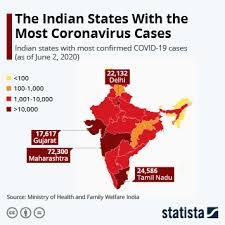
\includegraphics[width=7cm]{c19.jpg}
    \caption{Cases in India}
    \label{fig:enter-label}
\end{figure}
\begin{figure}[h]
    \centering
    
\includegraphics[width = 1.5cm]{cov.png}
    \caption{Stay informed}
    \label{fig:enter-label}
\end{figure}
\\
\textbf{Following is a Description type List}
\begin{description}
  \item[CS 213] Lorem ipsum dolor sit amet, consectetur adipiscing elit, sed do eiusmod tempor incididunt ut labore et dolore magna aliqua. Ut enim ad minim veniam, quis nostrud exercitation ullamco laboris nisi ut aliquip ex ea commodo.

  \item[HS 201] Lorem ipsum dolor sit amet, consectetur adipiscing elit, sed do eiusmod tempor incididunt ut labore et dolore magna aliqua. Ut enim ad minim veniam.
\end{description}

\newpage
\pagecolor{green}
\begin{table}[ht]
\centering
\begin{tabular}{|c|c|c|c|c|}
    \hline
    Names & \multicolumn{2}{c|}{maths} & \multicolumn{2}{c|}{science} \\ 
    \hline
    \multirow{2}{*}{Lorem} & X & Y & Z & W \\ \cline{2-5}
    & S & R & V & U	 \\ 
    \hline
    \multirow{2}{*}{Ipsum} & 3 & 2 & 0 & 1 \\ \cline{2-5}
    & T & O & P & Q \\
    \hline
    \multirow{2}{*}{Lorm} & A & B & C & D \\ \cline{2-5}
    & 2 & 3 & 1 & 0 \\
    \hline
\end{tabular}
\caption{Scores}
\end{table}
\section{Fonts}
Till now we have seen \textcolor{red}{mathematical formulae} in \colorbox{blue}{section 1} and \textcolor{red}{covid data} with figures and tables in \colorbox{blue}{section 2}. 
In \colorbox{blue}{section 3} we will use font properties. \begin{itemize}
\item Bold-\textbf{This text is bold}. 
\item Italics-\textit{This text is italic}. 
\item teletype-\texttt{This text is teletype}. 
\item emphasize-\emph{This text is emphasized}. 
\item Roman-\rm {This text is roman font family}. 
\item sans serif- \sf{This text is sans serif font family}.
\item slant-\sl{This text is slant}. 
\item small capital-\textsc{This text is small capital.} 
\item uppercase- THIS TEXT IS UPPERCASE. 
\item \text{lowercase- this text is lowercase.}
\end{itemize}
 The table 2 is a multi-column and multi-row table.

\newpage
\pagecolor{white}
\section{Psuedo Code}
\begin{algorithm2e}
\Function{QuickSort}{$A, p, r$}
    \If{$p < r$}
        \State $q \gets \text{Partition}(A, p, r)$
        \State \Call{QuickSort}{$A, p, q - 1$}
        \State \Call{QuickSort}{$A, q + 1, r$}
    \EndIf
\EndFunction

\Function{Partition}{$A, p, r$}
    \State $x \gets A[p]$ 
    \State $i \gets p - 1$
    \For{$j \gets p$ to $r - 1$}
        \If{$A[j] < x$}
            \State $i \gets i + 1$
            \State \Call{Swap}{$A[i], A[j]$}
        \EndIf
    \EndFor
    \State \Call{Swap}{$A[i + 1], A[r]$}
    \State \Return $(i + 1)$
\EndFunction
\end{algorithm2e}

The Algorithm is derived taking a hint from \cite{hoare1962quicksort}
 \newpage
 %\section{References}
\begin{thebibliography}{7}
\bibitem{verma2008concepts}
H. Verma, Concepts of Physics [Part 2], 2008.

\bibitem{education2016mathematics}
P. Education, \textit{The Mathematics Springboard 10th}, Pearson Education India, 2016.

\bibitem{ghorpade2018course}
S. R. Ghorpade and B. V. Limaye, \textit{A course in calculus and Real Analysis}, Springer, 2018.

\bibitem{huang2020treating}
M. Huang, T. Tang, P. Pang, M. Li, R. Ma, J. Lu, J. Shu, Y. You, B. Chen, J. Liang, et al., \emph{Treating COVID-19 with chloroquine}. \emph{Journal of Molecular Cell Biology}, vol. 12, no. 4, pp. 322–325, 2020.


\bibitem{hoare1962quicksort}
C. A. Hoare, Quicksort, \textit{The Computer Journal}, vol. 5, no. 1, pp. 10–16, 1962.

\end{thebibliography}
\end{document}